\chapter{Work Completed}\label{C:work}

\section{System Architecture \& Design}

\begin{itemize}
    
    \begin{figure}[H]
        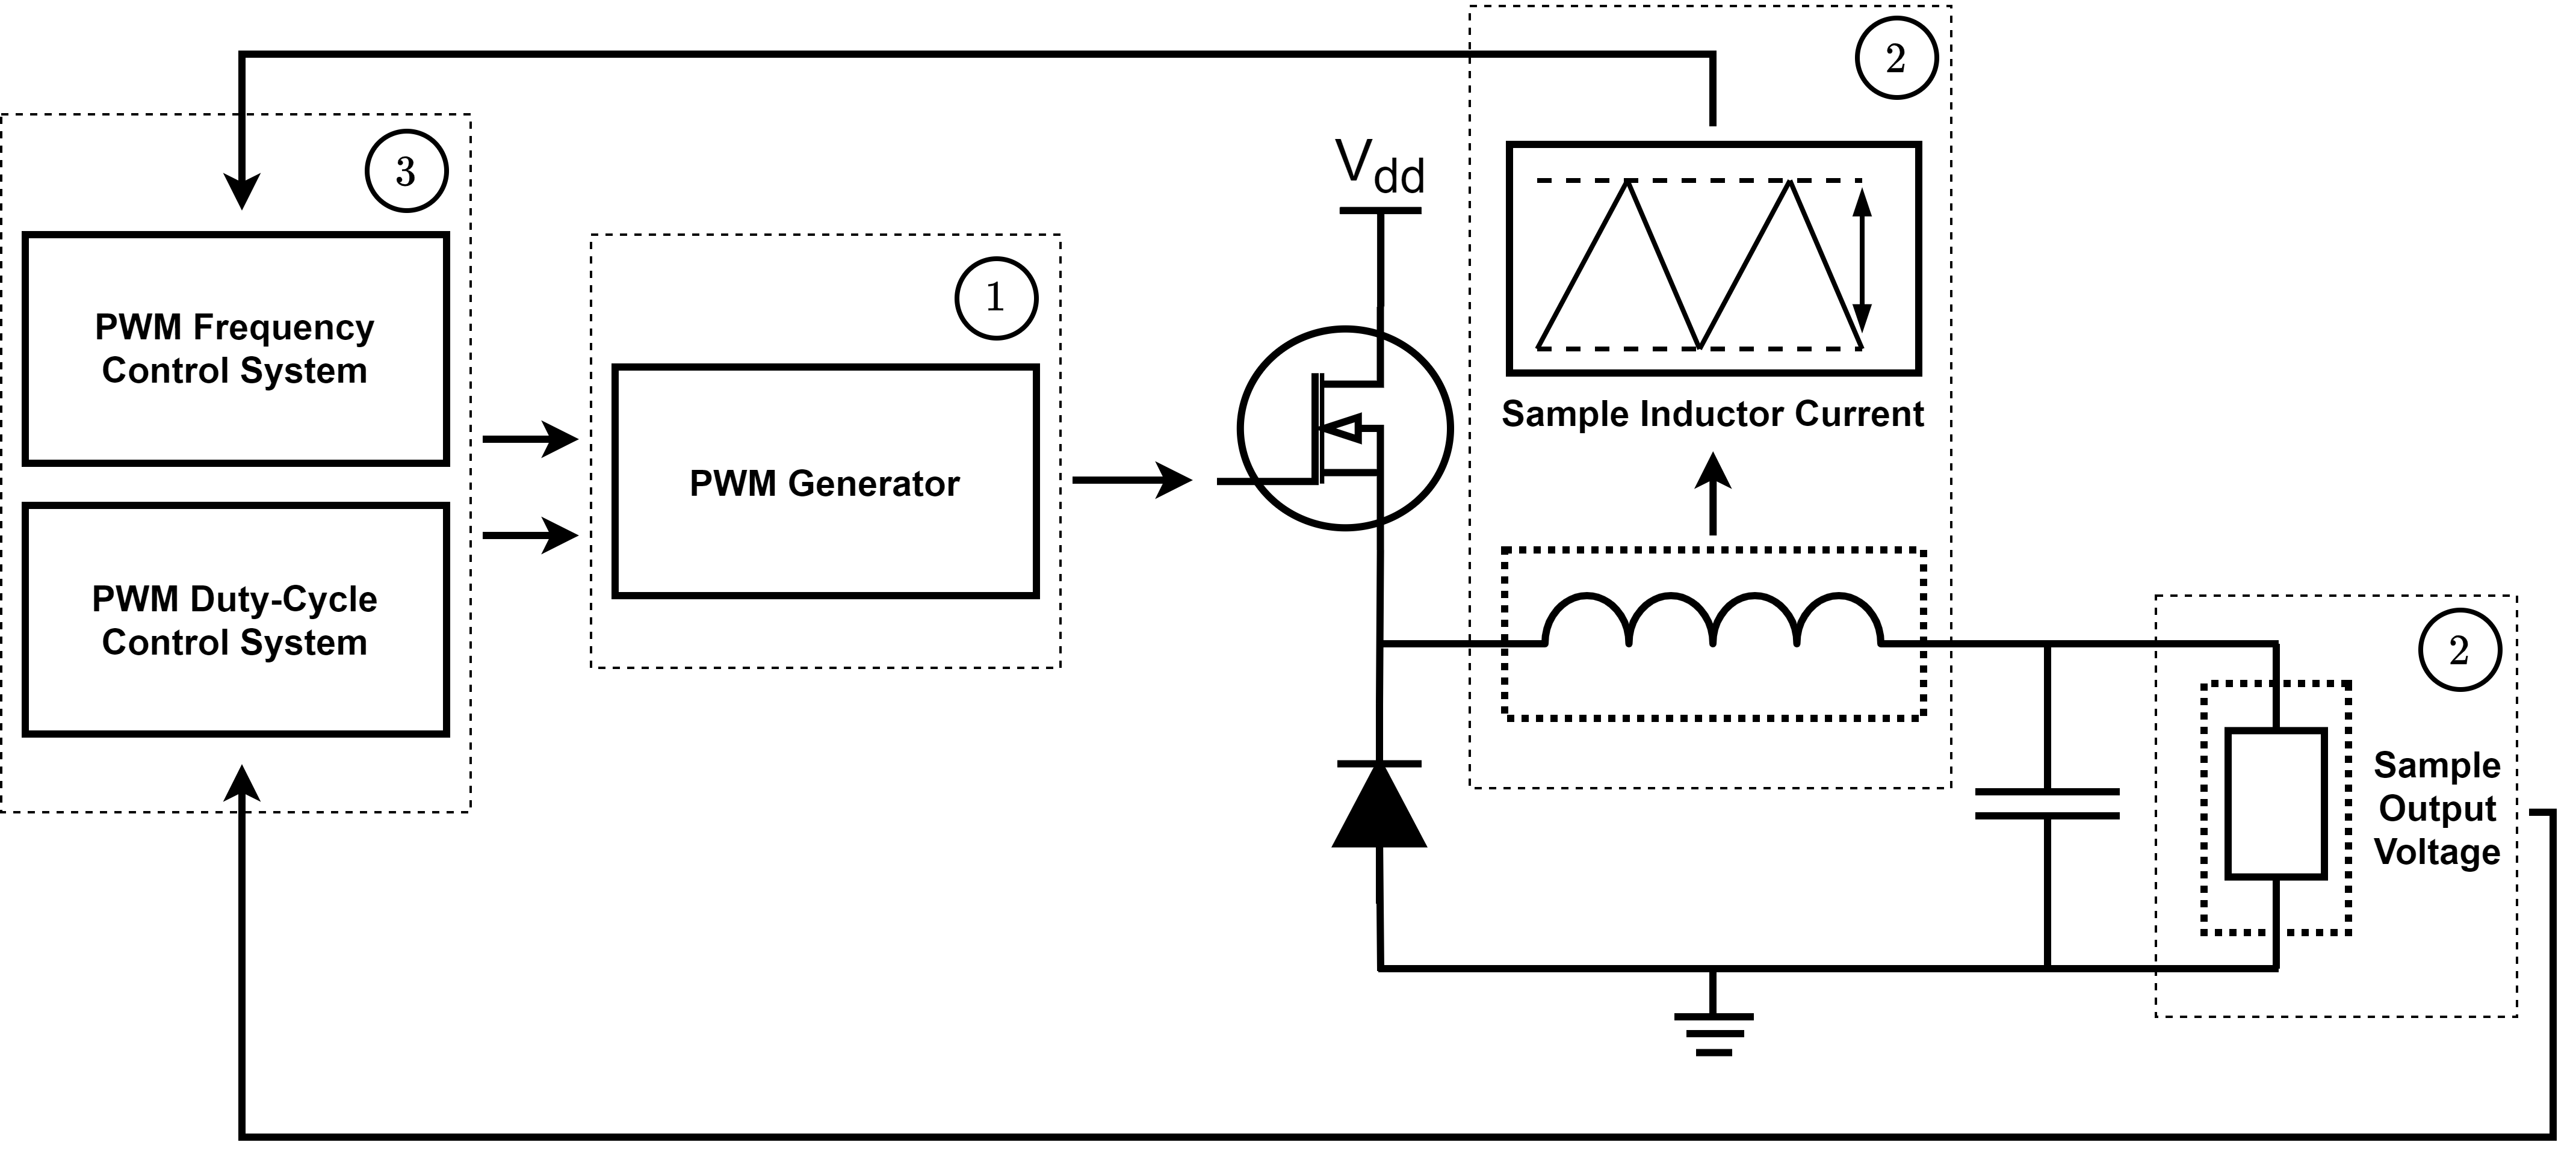
\includegraphics[width = 1\textwidth]{System_Overview.png}
        \caption{High level system overview}
        \label{F:sys_overview}
    \end{figure}

    \item 
    Give an overview of the entire system architecture. This means a high level block diagram of what different inputs and outputs are, and what the different signals in the system are. This can be done with the help of a diagram that I will create. 
    

\end{itemize}

\section{Defining \& Justifying System Specifications}

\begin{itemize}

    \item 
    Discuss the requirements that were laid out in the project proposal for the evaluation of the system. 

    \item 
    Discuss how these system requirements needed to be translated into a set of quantitative system requirements that can be used to define and design the system.
    
    \item 
    Discuss the system requirements that are required to effectively design the system (PWM frequency \& duty cycle step size), and then outline how they were calculated.
    
    \item 
    Discuss how these requirements will affect the design of the system

\end{itemize}

\section{PWM Generation Design}

\begin{itemize}

    \item 
    Discuss the different PWM generation methods outlined in chapter \ref{C:background}. Talk about each of their specific design implication, their advantages, and their disadvantages. This will be included in three different sections, analogue, microcontroller, FPGA. 

    \item 
    Discuss why I have selected a microcontroller for the PWM generation. And discuss how the design of this implementation affected the microcontroller selection. 

    \item 
    Discuss how the final design of the PWM generation was implemented, and what it's capabilities are. Show some images of it functioning, and attach the esp32 code in the appendix.

\end{itemize}